In this appendix we report the results of testing Particle Q-learning using the Double version of the algorithm, inspired from \cite{Hasselt:2016:DRL:3016100.3016191}. We tested the algorithms in the same domains described in Chapter \ref{chap:chapter5}, using the same experimental settings. Our PQL agents seem to be more unstable when used in their double version.
\subsubsection{Chain}
\begin{figure}[H]
 \includegraphics[width=\linewidth]{Chain/double_learning_curve.pdf}
 \caption{Online (left) and offline (right) scores for the double algorithms in the Chain domain.}
\end{figure}
\subsubsection{Loop}
\begin{figure}[H]
 \includegraphics[width=\linewidth]{Loop/double_learning_curve.pdf}
 \caption{Online (left) and offline (right) scores for the double algorithms in the Loop domain.}
\end{figure}
\subsubsection{Taxi}
\begin{figure}[H]
 \includegraphics[width=\linewidth]{Taxi/double_learning_curve.pdf}
 \caption{Online (left) and offline (right) scores for the double algorithms in the Taxi domain.}
\end{figure}
\subsubsection{River Swim}
\begin{figure}[H]
 \includegraphics[width=\linewidth]{RiverSwim/double_learning_curve.pdf}
 \caption{Online (left) and offline (right) scores for the double algorithms in the River Swim domain.}
\end{figure}
\subsubsection{Six Arms}
\begin{figure}[H]
 \includegraphics[width=\linewidth]{SixArms/double_learning_curve.pdf}
 \caption{Online (left) and offline (right) scores for the double algorithms in the Six Arms domain.}
\end{figure}
\subsubsection{Knight Quest}
\begin{figure}[H]
 \includegraphics[width=\linewidth]{KnightQuest/double_learning_curve.pdf}
 \caption{Online (left) and offline (right) scores for the double algorithms in the Knight Quest domain.}
\end{figure}